% Table A.2: its generator renders this table as an image only (no .md/.tex source), so the rendered page(s) are placed
% in a table environment. Copy the PDFs from figures/ alongside (named below).
\begin{table}[p]
\centering
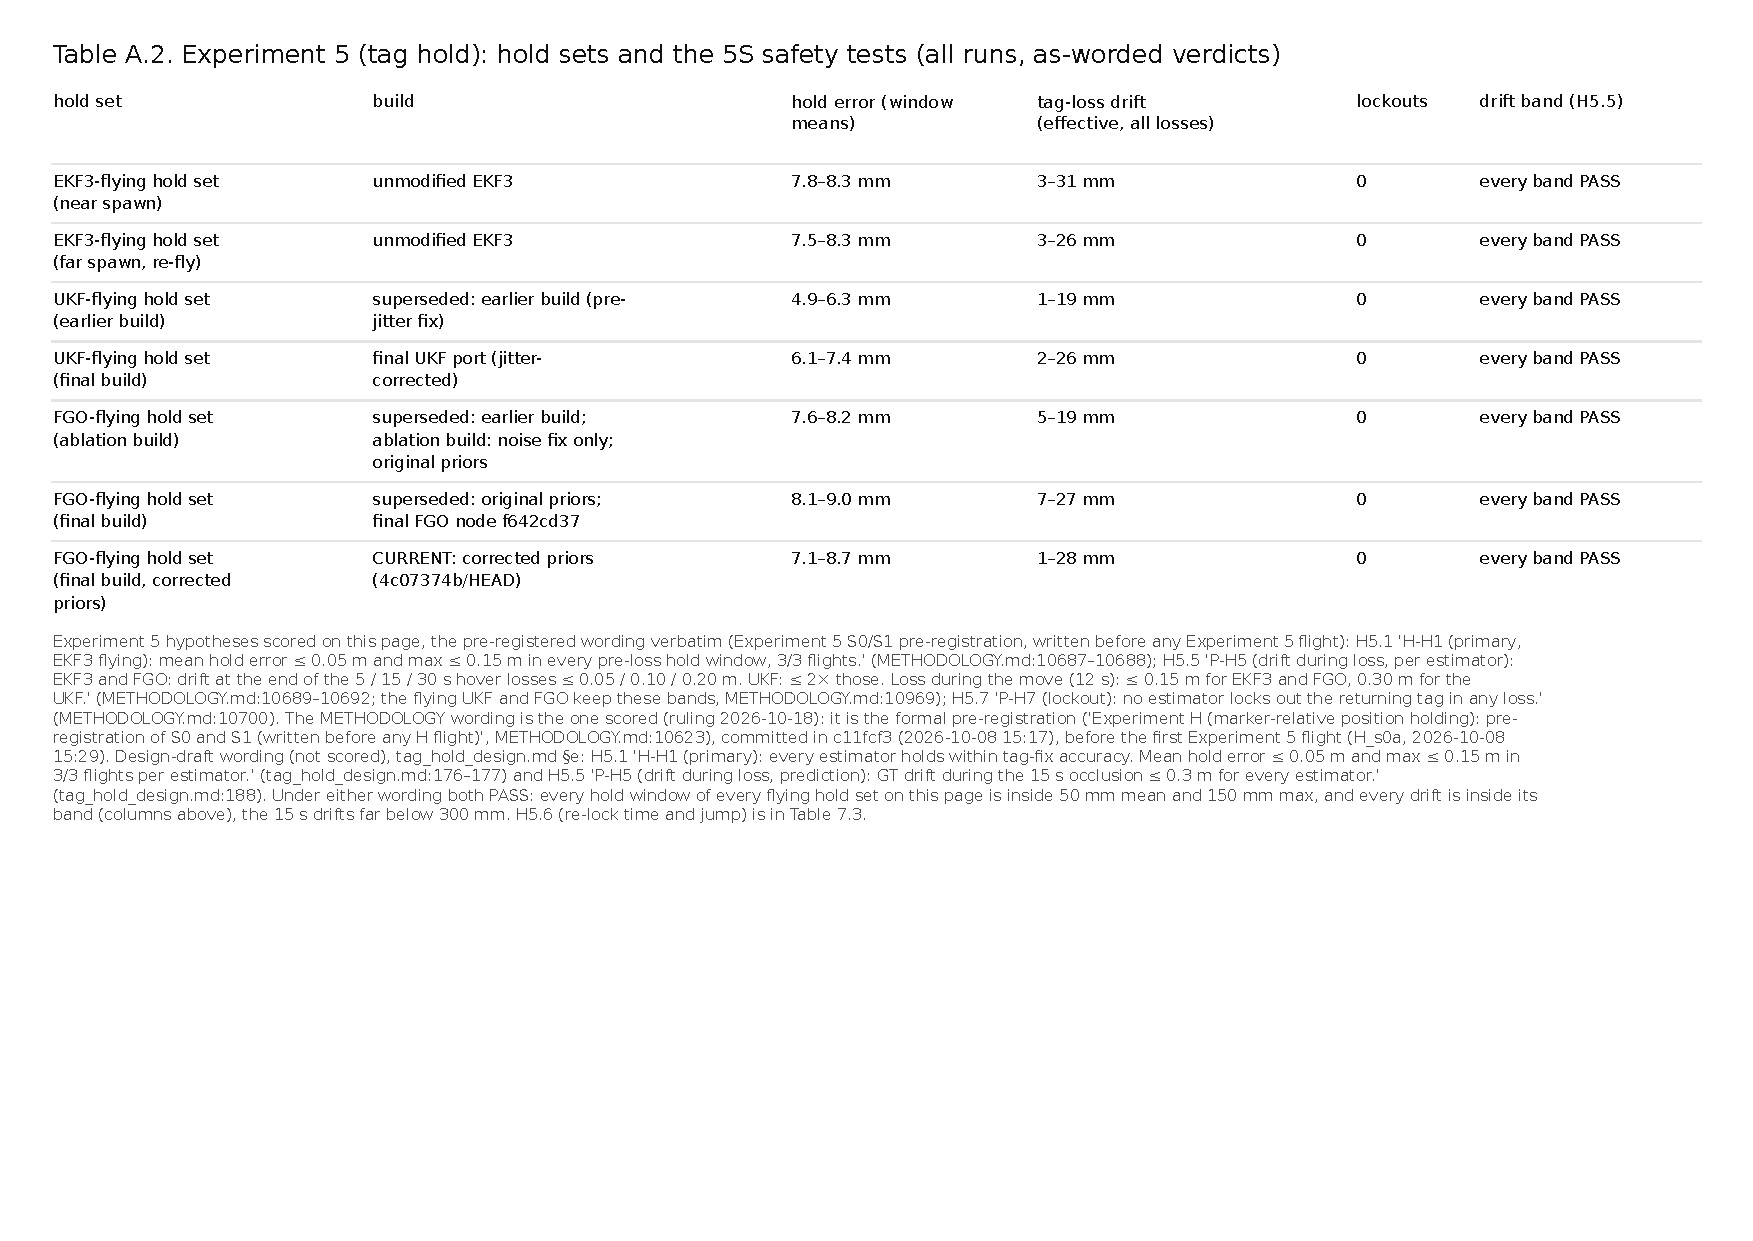
\includegraphics[width=\linewidth]{figures/tab_A-2_p1.pdf}\par\medskip
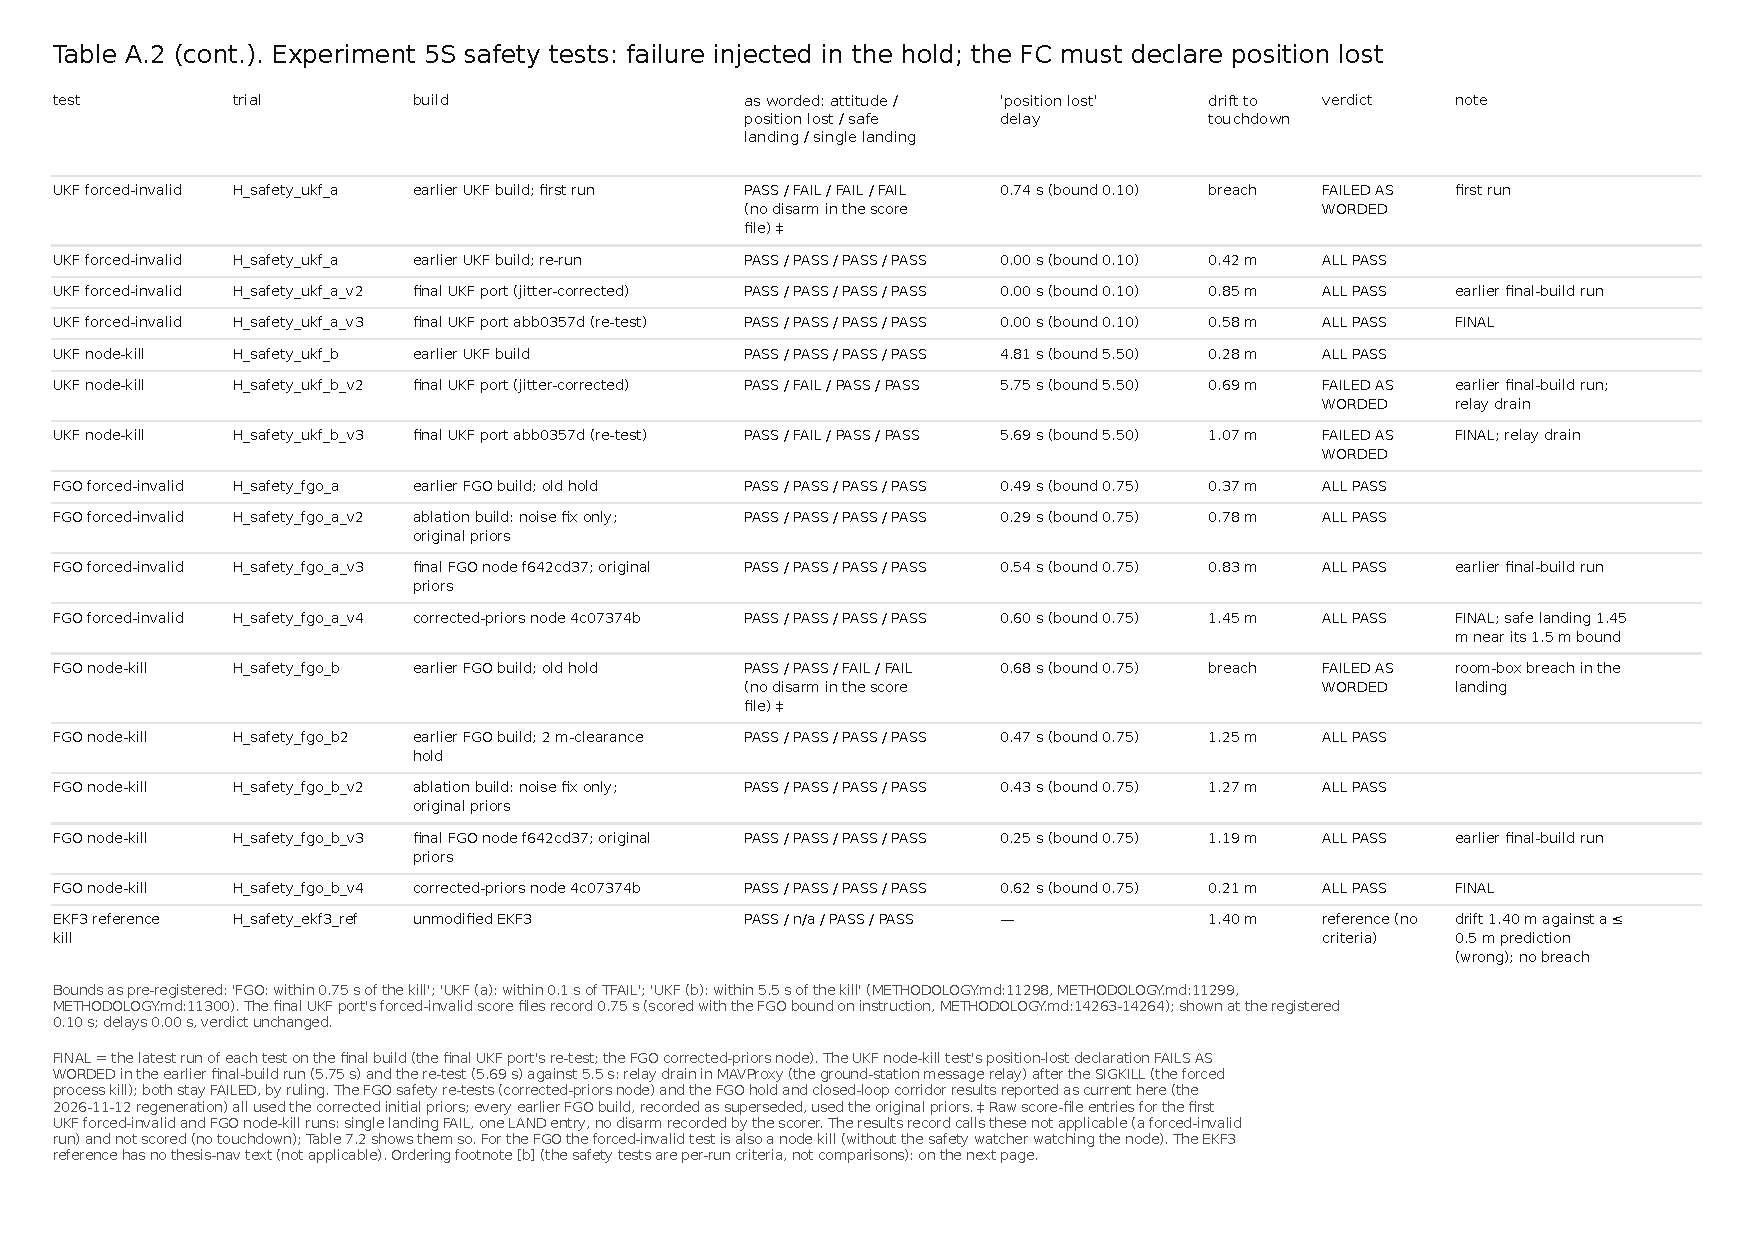
\includegraphics[width=\linewidth]{figures/tab_A-2_p2.pdf}\par\medskip
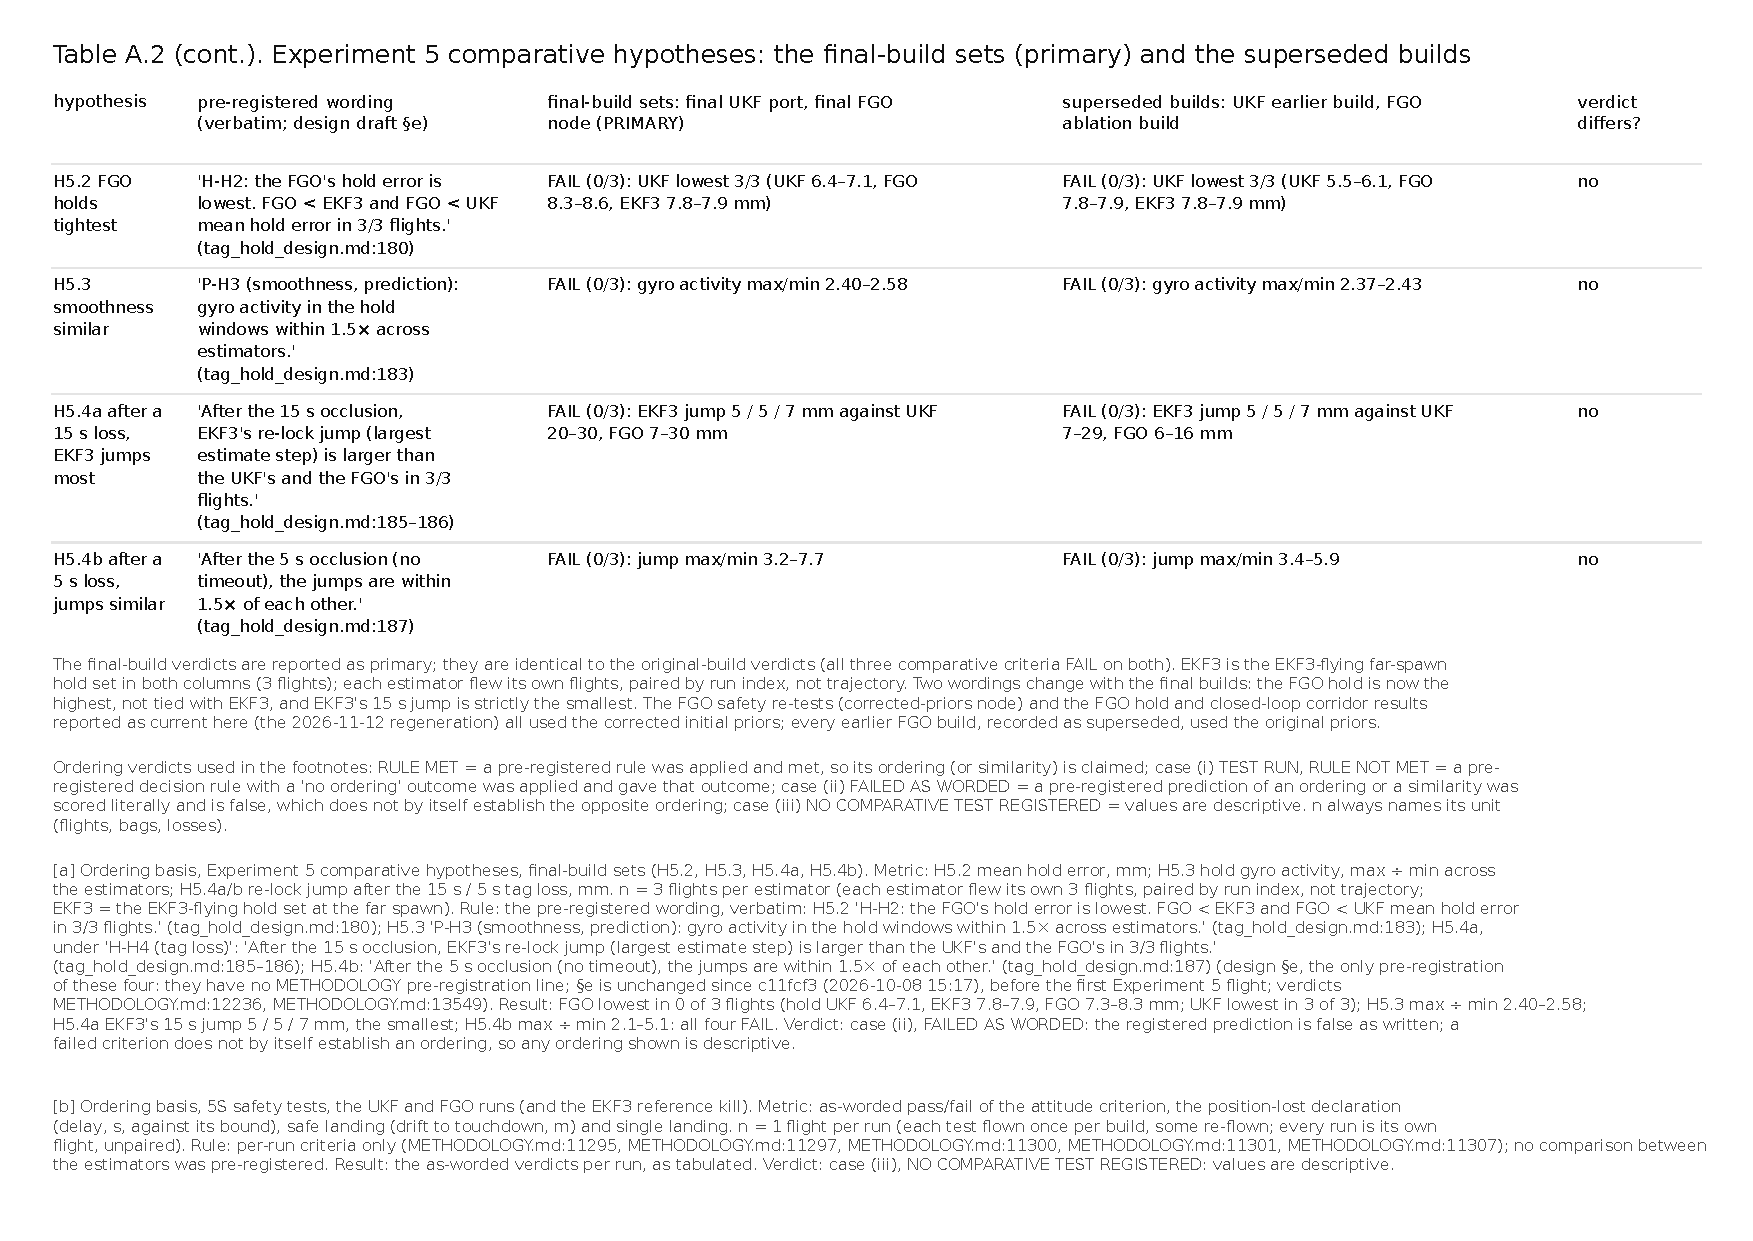
\includegraphics[width=\linewidth]{figures/tab_A-2_p3.pdf}\par\medskip
\caption{Table A.2. Experiment 5 hold sets and the 5S safety tests (all runs). Experiment 5 hold sets (EKF3-flying, near and far spawn; UKF-flying, earlier and final builds; FGO-flying, ablation and final builds) with hold error, drift, lockouts and the drift bands (H5.5), and every 5S safety-test run with its as-worded verdict; the final runs are the re-tests of the final UKF port and of the FGO corrected-priors node. The comparative criteria page gives this build-ablation record's own final-build sets beside the superseded earlier builds; the verdict category is identical in both and in the corrected-priors re-fly (all FAIL), though the FGO hold value narrows under the corrected priors [a]; the safety verdicts are per run [b]. Verdict rows (Table A.4, Experiment 5 and 5S): H5.1-H5.7 and the five 5S safety rows.}
\label{tab:A-2}
\end{table}
